\section{My Lower Back Can't Take It Anymore - How to Maintain Cervical and Lumbar Health}

\subsection{Relieving Back Problems: Standing Desk}

\begin{minipage}[t]{0.39\textwidth}
    \begin{figure}[H]
        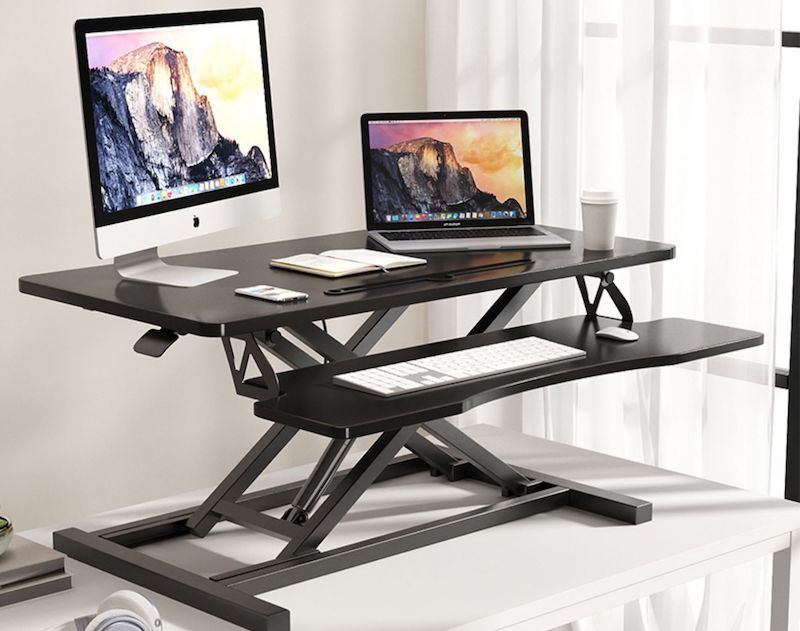
\includegraphics[width=0.95\columnwidth, right]{author-folder/Yue.Zhou/gongzuotai.jpg}
    \end{figure}
\end{minipage}
\begin{minipage}[t]{0.6\textwidth}
    Before pursuing my PhD, I already had severe lumbar muscle strain. This condition, while not a major illness, constantly torments you. At its worst, the pain kept me awake at night. I visited the hospital and got medication, but the doctor said this condition requires self-care and cannot be completely cured. Later, I tried running for half a year, and miraculously, the lumbar muscle strain improved, and now it doesn't hurt at all (though prolonged sitting still causes pain). After starting my PhD, I lost the motivation to exercise, so I bought a standing desk (highly recommended for everyone! It's so useful!). You can work standing up, and when you get tired, you can sit down. This greatly reduces the damage to the lumbar spine caused by prolonged sitting.
\end{minipage}

\begin{flushright}
(December 30, 2022 by Yue Zhou)

Translated by GPT
\end{flushright}

\subsection{In-depth Advice from a Severe Lumbar Disc Herniation and Cervical Spondylosis Patient}

\subsubsection{Standing Desk: Can Greatly Relieve Lumbar Problems, But Not Completely Solve Them}

I've had lumbar disc herniation for ten years and cervical spondylosis for five years. In 2019, my back pain was so severe that I couldn't sit for a whole day, so I put a standing desk in the lab and used it for three years. This year, I also put the same standing desk in my bedroom. However, standing for long periods is just as bad for your back as sitting, and eventually, standing and sitting will both cause back pain. A standing desk is not a long-term solution; standing just changes the angle of stress on the lumbar spine.

You can't rely entirely on a standing desk: Over the years, I've relied too much on the standing desk, and now standing for long periods causes back pain just like sitting. When I went for an MRI, the doctor even asked if my back was fractured. To really relieve back pain, you need to avoid prolonged sitting and standing. High school teachers often suffer from back pain partly because they stand for long periods while teaching.

In summary, a standing desk can be used, but it shouldn't replace sitting at a computer for long periods. Alternate between standing and sitting, and exercise regularly.

Note: Remember to adjust the height of the standing desk occasionally. The standing desk I put in the lab hasn't been adjusted for years, and it seems the hydraulic rod has rusted and won't move, turning it into a regular desk.

\subsubsection{External Monitor: Avoid and Relieve Cervical Spondylosis}

The uncomfortable thing about cervical spondylosis is that prolonged looking down causes neck pain. When I'm out on the subway or high-speed train, I have to hold my phone up to eye level, or I can't use it for long.

Another way to avoid and relieve cervical spondylosis is to avoid using a laptop for long periods. Prolonged looking down at the screen can lead to cervical spondylosis. The same goes for looking down at your phone.

If you use a laptop frequently, place a desktop monitor in both your bedroom and office as an external monitor.

I developed cervical spondylosis after a year of intensive laptop use, and it stopped worsening after I switched to using an external monitor.

If you frequently use a laptop intensively without an external monitor, it's just as bad for your neck as looking down at your phone all day. I often advise people in the lab who use laptops for long periods to use an external monitor.

A laptop stand can also help and is cheaper than a monitor. But if you have poor eyesight, it's better to use an external monitor because laptop screens are too small and strain your eyes. I used to buy many laptop stands, but now I use them to hold monitors, and the laptop fits nicely underneath.

\begin{figure}[H]
    \caption{In my bedroom, I use a standing desk with a laptop stand. This combination works well for someone like me who mainly uses a laptop.}
    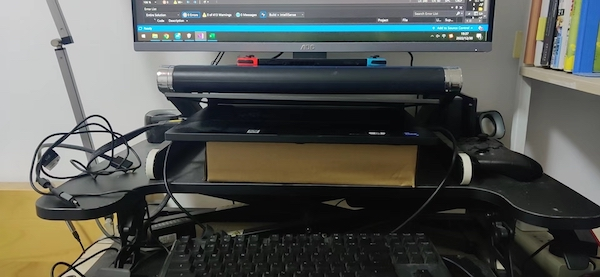
\includegraphics[width=0.95\columnwidth, center]{author-folder/Jialin.Wang/shengjiangzhuo.jpeg}
\end{figure}

% \subsubsection{Further Relief: Using the Computer While Lying Down}

% Since the beginning of this year, I can't stand for long periods, so I've started exploring using the computer while lying down or prone. I tried lying down for a few days but gave up because it made me sleepy. I think lying down is more suitable for watching movies or playing games.

% I've been trying the prone position for a month now, and it feels okay. At least propping up my upper body doesn't make me sleepy.

% I placed a portable monitor by the bed and used a prone pillow, which allows me to lie down all day. The prone pillow is great because it doesn't compress the abdomen after meals, causing discomfort.

% \begin{figure}[H]
%     % \centering
%     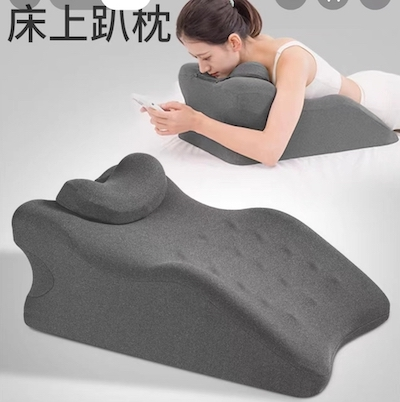
\includegraphics[width=0.3\columnwidth, center]{author-folder/Jialin.Wang/pazhen.jpeg}
% \end{figure}

% Then I use an adjustable laptop stand for the monitor, keyboard, and mouse—though you can just use a laptop, but it's inconvenient due to the heat and moving it around. A portable monitor allows quick switching between the standing desk and prone position—I also considered buying a regular monitor stand, but there aren't any suitable for bed use, and regular monitors are too big for bed use. A portable monitor, which is a repurposed laptop screen, is just the right size for bed use.

% If you use the computer while lying down for long periods, I found it's best to use your arms to slightly support your upper body. But the main support should come from the torso, with the arms providing auxiliary support to avoid too much pressure on the chin.

% I've now mastered the ability to lie prone all day. As long as the laptop stand is adjusted to the right angle, keeping the hands and arms parallel, the wrists won't get sore from prolonged bending.

% However, since I've gotten used to lying down and it's cold, I don't exercise at all. If I don't lie down, my back still hurts. Regular exercise is essential.

% This setup is perfect for someone like me who can't sit or stand for long periods due to back pain, but it won't cure the pain. Exercise is the most important thing. Without regular exercise, unused muscles will atrophy, making things worse. (I wish I could live in a tropical coastal area and swim at the beach every evening; the sea water is warm in the evening.)

\subsubsection{The Best Solution: Change Lifestyle Habits and Exercise More}

For those with lumbar disc herniation and cervical spondylosis, regular exercise is recommended. But don't blindly go to the gym; the best exercise is swimming because most other exercises require using the back muscles, which can worsen the pain.

Currently, I only occasionally have back pain that prevents me from bending over. I know someone whose back pain was so severe that they walked with a limp, but they gradually improved through exercise.

If you lack self-discipline, joining a school swimming club can help, as having people to exercise with regularly can be motivating.

If you get a membership, I remember the Dushu Lake Swimming Pool offers half-price annual memberships every September, but school clubs are cheaper and more cost-effective. Before I got a swimming membership, I used to go swimming once or twice a week with the school swimming club. After getting the annual membership, I went less than five times a year, and even less frequently afterward.
If you have self-discipline, daily exercise is the best method.
If you can't stick to it and can't change your lifestyle habits, the condition will worsen.

Finally, if the back pain is severe, visit the hospital's orthopedics department for an MRI to see the extent of the lumbar spine condition and determine the specific recovery plan. Back pain is now common among young people.

\begin{flushright}
(December 30, 2022 by Jialin Wang)

Translated by GPT
\end{flushright}
